% =============================================================
% Capítulo 9 - Desarrollo del software de interfaz (HMI)
% =============================================================
\chapter{Desarrollo del software de interfaz (HMI)}
\label{cap:software_hmi}
% El capítulo del firmware referencia a éste como \ref{cap:hmi}. Si preferís una
% sola etiqueta, borrá la línea siguiente y cambiá esa referencia allá.
\label{cap:hmi}

El software de interfaz hombre-máquina (HMI, por sus siglas en inglés \emph{Human-Machine Interface}) constituye la capa de supervisión y control del sistema automatizado de sintonización en longitud de onda para el HSRL. Este desarrollo reemplaza el esquema previo basado scripts en Visual C++ por una solución integrada, robusta y amigable para el operador.


El software HMI debe permitir la interacción entre el usuario y el microcontrolador de la placa de control, incluyendo la visualización del estado de sintonización del sistema, la lectura de parámetros del lazo de control y la modificación de funciones y \emph{setpoints} de operación.

\section{Requisitos funcionales y de diseño}
\label{sec:reqhmi}

Para garantizar la operabilidad, confiabilidad y seguridad del sistema, se establecieron los siguientes requisitos funcionales y de diseño específicos:

\begin{itemize}
    \item \textbf{Monitoreo en tiempo real:} Visualización continua del estado operativo de sintonización (sintonizando, bloqueado en longitud de onda, fuera de rango o error), así como el despliegue gráfico de las señales adquiridas por los detectores de pico ($P_+$ y $P_-$), el valor de error del lazo $e(k)$ y el valor de salida del actuador de temperatura $T(k)$.
    \item \textbf{Control y configuración de parámetros:} Permitir al usuario modificar dinámicamente los parámetros del lazo de control de banda muerta, enviar valores consigna (\emph{setpoints}), seleccionar modos de operación (Manual / Automático) y enviar comandos de control a la placa de control.
    \item \textbf{Gestión de alarmas e incidencias:} Notificación inmediata y clara ante desvíos de los parámetros de sintonización, pérdidas de señal pulsada, fallas de comunicación o sobrepasos de umbrales en los fotodetectores.
    \item \textbf{Registro de datos (Data Logging):} Almacenamiento periódico de la telemetría del sistema y eventos en archivos de registro (\emph{log files}) para su posterior análisis meteorológico y diagnóstico técnico.
\end{itemize}

Si bien no es requisito utilizar una norma puntual, se considera como una buena práctica seguir estándares probados, por lo tanto el diseño toma como base los lineamientos de la norma ISA-101 introducidos en la Sección~\ref{sec:isa101} y el principio de alarmas de la ISA 18.2, introducido en la Sección~\ref{sec:alarmas}.

\section{Principios de la norma ISA-101}
\label{sec:isa101}

La norma ANSI/ISA-101.01-2015 (\emph{Human Machine Interfaces for Process Automation Systems}) establece directrices de diseño orientadas a maximizar la conciencia situacional (\emph{situation awareness}) del operador, reducir el tiempo de respuesta ante eventos anómalos y minimizar la fatiga visual. Para la implementación del HMI del sistema HSRL se adoptaron los siguientes principios fundamentales de la norma \cite{isa101}

\begin{enumerate}
    \item \textbf{Filosofía de color simplificada y funcional:} se emplean fondos neutros en tonos de gris claro para los paneles y ventanas principales, evitando contrastes elevados que generen cansancio visual durante jornadas prolongadas de medición. El uso de colores vivos se reserva exclusivamente para la representación de estados de alarma o advertencias (rojo para fallas críticas, amarillo/ámbar para advertencias y verde o gris neutro para estados normales de operación).
    \item \textbf{Jerarquía estructurada de pantallas:} se define una distribución organizada del contenido funcional dividida en áreas bien delimitadas:
    \begin{itemize}
        \item \emph{Barra de estado superior (Header):} muestra el estado global de conexión serie, modo de operación actual (Manual/Automático) y el indicador sintético de sintonización (\emph{LOCKED/UNLOCKED}).
        \item \emph{Panel de proceso y gráficos en tiempo real:} despliega tendencias temporales de las señales $P^+$, $P^-$ y la señal de error $e(k)$, permitiendo evaluar la estabilidad del lazo de control de un solo vistazo.
        \item \emph{Panel de comandos y ajustes:} agrupa los controles interactivos para ingresar consignas, modificar el punto de operación y modo.
    \end{itemize}
\end{enumerate}

\section{Alarmas del sistema}
\label{sec:alarmas}

La gestión de alarmas se diseñó siguiendo los principios de la norma ANSI/ISA-18.2 (\emph{Management of Alarm Systems for the Process Industries}). El objetivo es garantizar que cada alarma presentada al operador responda a una condición anómala real que requiera una acción o toma de decisión consciente, evitando el fenómeno de desensibilización por saturación de alarmas (\emph{alarm flooding}). \cite{isa182}

Las alarmas del HMI se categorizan en dos niveles de prioridad:

\begin{itemize}
    \item \textbf{Prioridad Alta:} condición que compromete el funcionamiento del sistema o la integridad de la medición (por ejemplo, pérdida total de pulsos en los fotodetectores, error de comunicación serie prolongado o desenganche crítico del lazo). Requiere atención inmediata del operador. Representación en rojo.
    \item \textbf{Prioridad Media:} desviaciones temporales de la señal de error $e(k)$ por encima de los umbrales de tolerancia preestablecidos, o variaciones térmicas drásticas en el actuador $T(k)$. Representación en amarillo/ámbar.
\end{itemize}

\section{Modelo de HMI}

A partir de los criterios establecidos en la Sección \ref{sec:reqhmi} y las normas discutidas en las Secciones \ref{sec:isa101} y \ref{sec:alarmas} se creó el borrador de HMI presentado en la Figura \ref{fig:inks}, con los botones y comandos necesarios para la operación de sistema, utilizando el software Inkscape.

\begin{figure}
    \centering
    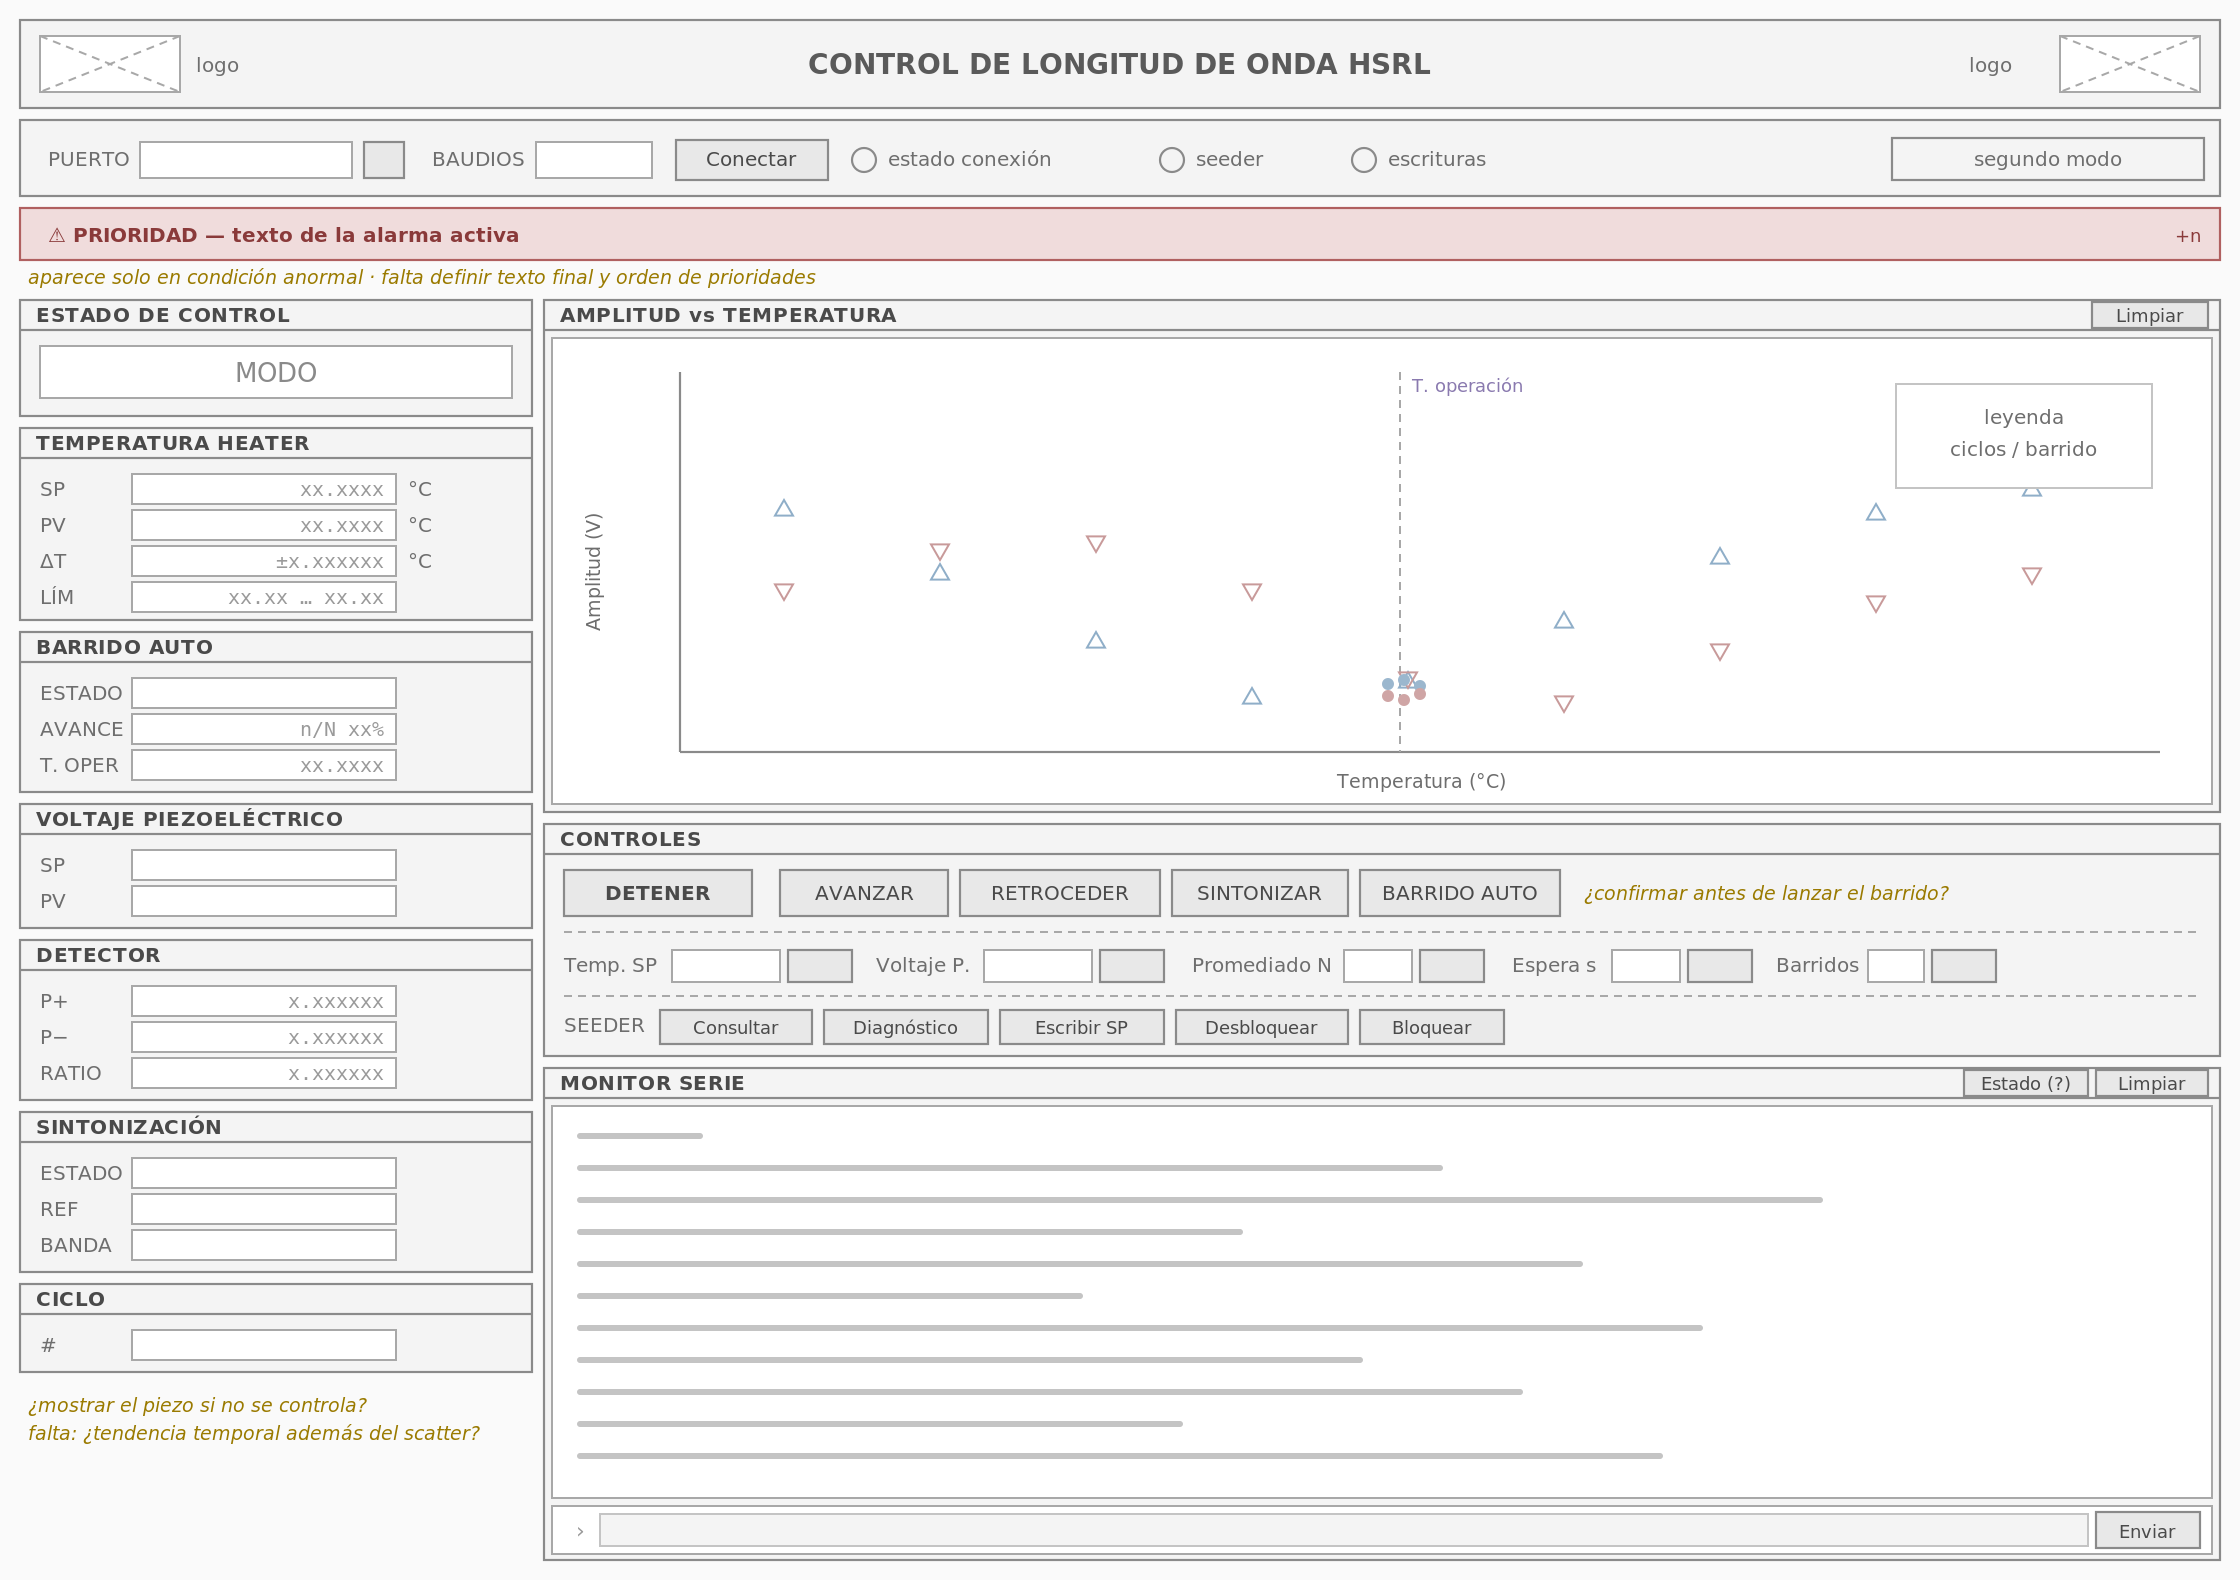
\includegraphics[width=0.8\textwidth]{figuras/8_borradorhmi.png}
    \caption{Borrador del HMI creado en Inkscape (Fuente: elaboración propia).}
    \label{fig:inks}
\end{figure}

\section{Arquitectura del software en Python}
\label{sec:arquitectura_python}
\label{sec:hmi-arquitectura}

Se implementó el HMI en Python, con Tkinter para la interfaz gráfica. El código fuente se documenta y versiona en el repositorio del proyecto. La aplicación tiene exactamente dos dependencias externas fundamentales: \texttt{pyserial} para la comunicación por puerto USB con la placa de control y \texttt{matplotlib} para la representación gráfica; Tkinter forma parte de la biblioteca estándar. Se organiza en siete módulos, según muestra la Figura~\ref{fig:hmi-modulos}.


\begin{figure}[htbp]
    \centering
    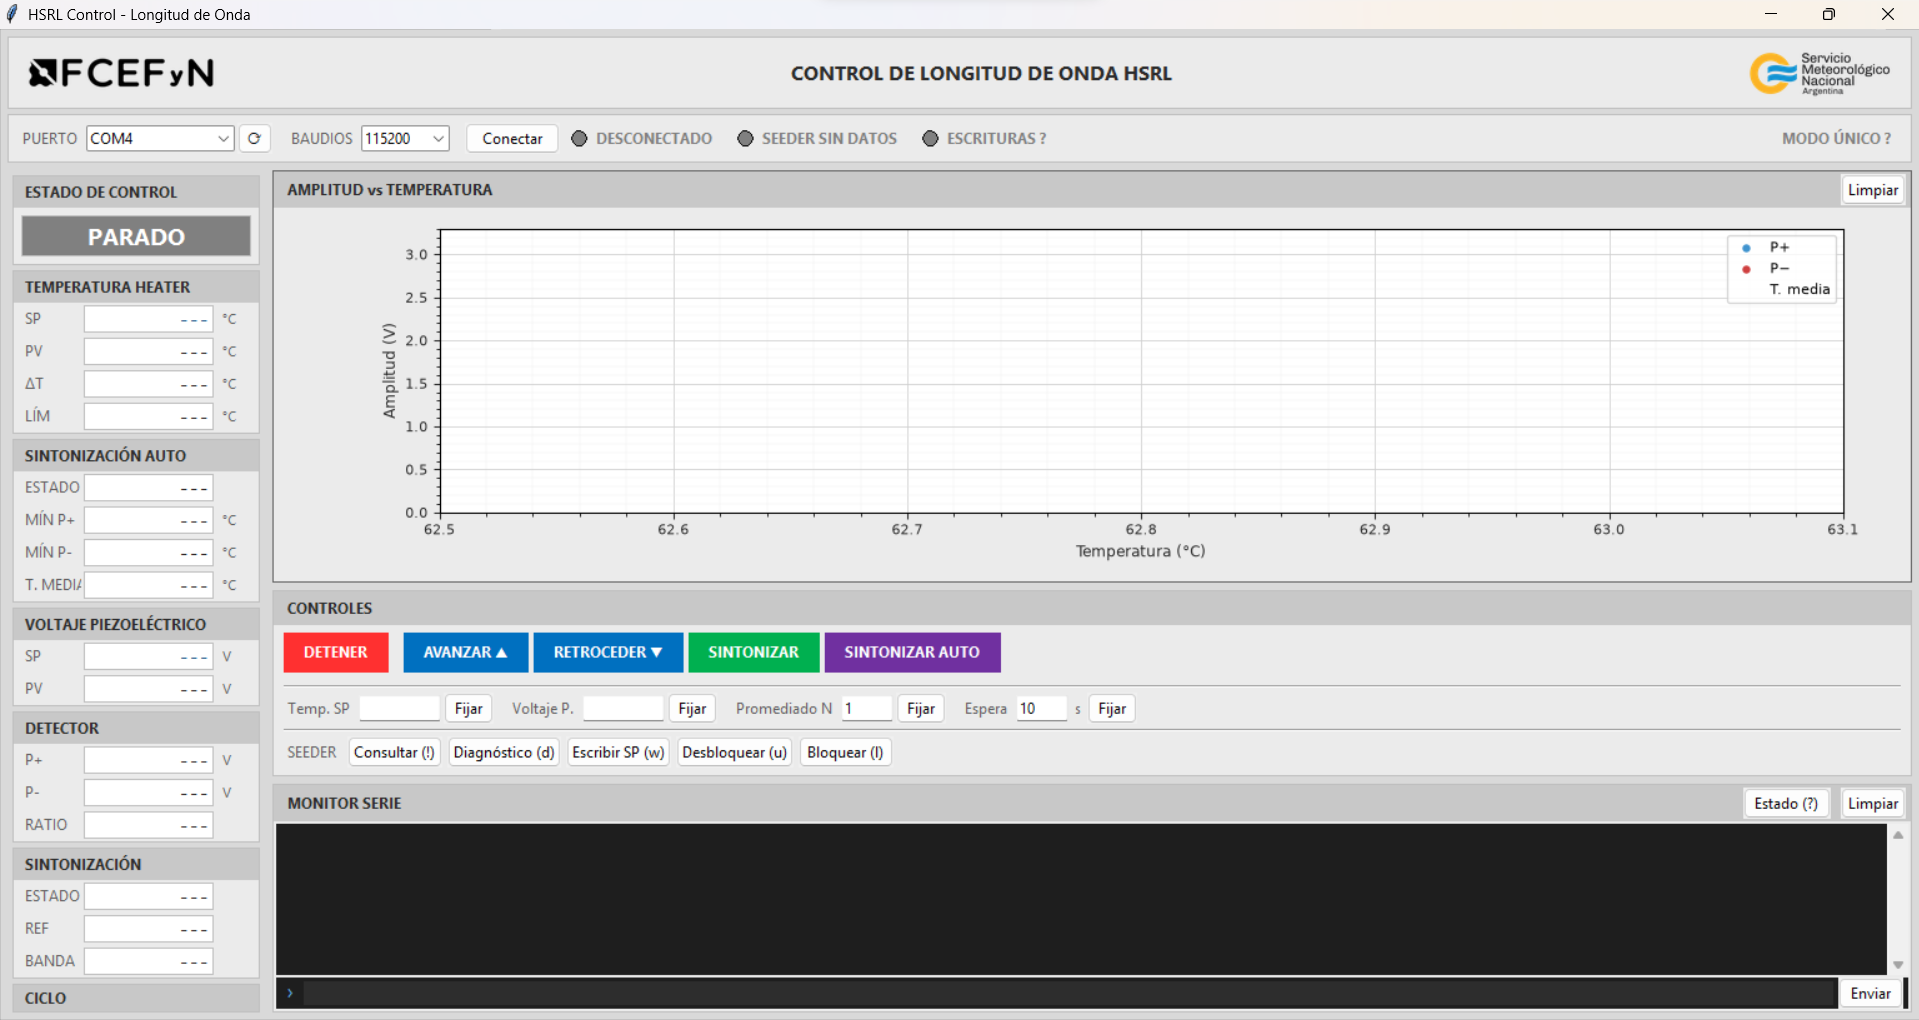
\includegraphics[width=0.8\textwidth]{figuras/8_hmilayout.png}
    \caption{HMI generado por hmi.py, a partir de la referencia proporcionada a Opus 4.7 (Fuente: elaboración propia).}
    \label{fig:hmiopus}
\end{figure}

La base de los módulos \texttt{hmi.py} y \texttt{serie.py} fueron creados a partir del uso del modelo de IA Opus 4.7, con el prompt \"crear HMI a partir de la imagen de borrador proporcionado. Cada comando de la recepción mediante pySerial debe interactuar con el firmware proporcionado con sus respectivos botones y campos de E/S\". Luego fueron modificados y adaptados según la necesidad del proyecto. Los archivos proporcionados de referencia para el modelo fueron el borrador de la Figura \ref{fig:inks} y los archivos \emph{hsrl-control.c} y \emph{config.h}.

\begin{figure}[htbp]
\centering
\resizebox{\textwidth}{!}{% Figura: hmi-modulos -- requiere % =====================================================================
%  Estilos compartidos por los diagramas TikZ de los capitulos.
%  Va en el PREAMBULO del documento principal:
%      % =====================================================================
%  Estilos compartidos por los diagramas TikZ de los capitulos.
%  Va en el PREAMBULO del documento principal:
%      \input{diagramas/estilos-diagramas}
% =====================================================================

\usepackage{tikz}
\usepackage{amsmath}
\usepackage{amssymb}
\usetikzlibrary{arrows.meta,positioning,shapes.geometric,shapes.misc,calc,fit,backgrounds,decorations.pathreplacing}

\definecolor{cbloque}{HTML}{E8EEF4}
\definecolor{cborde}{HTML}{4A6D8C}
\definecolor{cacento}{HTML}{D9E6D5}
\definecolor{cacentob}{HTML}{5A7A4A}
\definecolor{cgris}{HTML}{EDEDED}
\definecolor{cgrisb}{HTML}{888888}
\definecolor{calarma}{HTML}{F6DEDE}
\definecolor{calarmab}{HTML}{A03030}

\tikzset{
  bloque/.style={draw=cborde,fill=cbloque,rounded corners=2pt,align=center,
                 inner sep=5pt,font=\footnotesize,minimum height=9mm},
  bloqueg/.style={bloque,draw=cgrisb,fill=cgris},
  bloquea/.style={bloque,draw=cacentob,fill=cacento},
  bloquer/.style={bloque,draw=calarmab,fill=calarma},
  proceso/.style={bloque,minimum width=52mm},
  decision/.style={draw=cborde,fill=cbloque,align=center,font=\scriptsize,
                   diamond,aspect=2.2,inner sep=1pt},
  flecha/.style={-{Stealth[length=2mm]},draw=cborde!80!black,thick},
  flechag/.style={flecha,draw=cgrisb},
  et/.style={font=\scriptsize,inner sep=1.5pt,fill=white,align=center},
  etl/.style={et,midway},
  grupo/.style={draw=cgrisb,dashed,rounded corners=3pt,inner sep=4mm},
  tit/.style={font=\scriptsize\bfseries,text=cgrisb!60!black},
}

% --- utilidades para diagramas de secuencia ---
\tikzset{
  vida/.style={draw=cgrisb,dash pattern=on 2pt off 2pt},
  cab/.style={bloque,minimum width=26mm,font=\scriptsize\bfseries},
  nota/.style={draw=cacentob,fill=cacento,font=\scriptsize,align=center,
               rounded corners=1pt,inner sep=3pt},
}
\newcommand{\msg}[4]{\draw[flecha] (#1,#3) -- (#2,#3) node[et,midway,above=0pt]{#4};}
\newcommand{\msgr}[4]{\draw[flecha,dashed] (#1,#3) -- (#2,#3) node[et,midway,above=0pt]{#4};}
\newcommand{\auto}[3]{%
  \draw[flecha] (#1,#2) -- ++(0.55,0) -- ++(0,-0.42) -- (#1,{#2-0.42});
  \node[et,anchor=west] at ({#1+0.7},{#2-0.21}) {#3};}


% =====================================================================

\usepackage{tikz}
\usepackage{amsmath}
\usepackage{amssymb}
\usetikzlibrary{arrows.meta,positioning,shapes.geometric,shapes.misc,calc,fit,backgrounds,decorations.pathreplacing}

\definecolor{cbloque}{HTML}{E8EEF4}
\definecolor{cborde}{HTML}{4A6D8C}
\definecolor{cacento}{HTML}{D9E6D5}
\definecolor{cacentob}{HTML}{5A7A4A}
\definecolor{cgris}{HTML}{EDEDED}
\definecolor{cgrisb}{HTML}{888888}
\definecolor{calarma}{HTML}{F6DEDE}
\definecolor{calarmab}{HTML}{A03030}

\tikzset{
  bloque/.style={draw=cborde,fill=cbloque,rounded corners=2pt,align=center,
                 inner sep=5pt,font=\footnotesize,minimum height=9mm},
  bloqueg/.style={bloque,draw=cgrisb,fill=cgris},
  bloquea/.style={bloque,draw=cacentob,fill=cacento},
  bloquer/.style={bloque,draw=calarmab,fill=calarma},
  proceso/.style={bloque,minimum width=52mm},
  decision/.style={draw=cborde,fill=cbloque,align=center,font=\scriptsize,
                   diamond,aspect=2.2,inner sep=1pt},
  flecha/.style={-{Stealth[length=2mm]},draw=cborde!80!black,thick},
  flechag/.style={flecha,draw=cgrisb},
  et/.style={font=\scriptsize,inner sep=1.5pt,fill=white,align=center},
  etl/.style={et,midway},
  grupo/.style={draw=cgrisb,dashed,rounded corners=3pt,inner sep=4mm},
  tit/.style={font=\scriptsize\bfseries,text=cgrisb!60!black},
}

% --- utilidades para diagramas de secuencia ---
\tikzset{
  vida/.style={draw=cgrisb,dash pattern=on 2pt off 2pt},
  cab/.style={bloque,minimum width=26mm,font=\scriptsize\bfseries},
  nota/.style={draw=cacentob,fill=cacento,font=\scriptsize,align=center,
               rounded corners=1pt,inner sep=3pt},
}
\newcommand{\msg}[4]{\draw[flecha] (#1,#3) -- (#2,#3) node[et,midway,above=0pt]{#4};}
\newcommand{\msgr}[4]{\draw[flecha,dashed] (#1,#3) -- (#2,#3) node[et,midway,above=0pt]{#4};}
\newcommand{\auto}[3]{%
  \draw[flecha] (#1,#2) -- ++(0.55,0) -- ++(0,-0.42) -- (#1,{#2-0.42});
  \node[et,anchor=west] at ({#1+0.7},{#2-0.21}) {#3};}

 en el preambulo
\begin{tikzpicture}[x=1cm,y=1cm]

\node[bloque,text width=62mm] (hmi) at (2.0,3.2)
  {\texttt{hmi.py}\\[1pt]\scriptsize \texttt{HmiApplication}: construcción de la pantalla,
   \texttt{\_poll\_serial()} cada 100\,ms, secuencia de sintonización automática};

\node[bloque,text width=34mm] (ser) at (-5.4,0.5)
  {\texttt{serie.py}\\[1pt]\scriptsize \texttt{SerialLink}: hilo lector,\\cola de líneas, \texttt{SerialLinkError}};
\node[bloque,text width=36mm] (tel) at (-0.4,0.5)
  {\texttt{telemetria.py}\\[1pt]\scriptsize \texttt{ProcessData} + \texttt{parse\_line()}\\(no importa Tkinter)};
\node[bloque,text width=32mm] (reg) at (4.4,0.5)
  {\texttt{registro.py}\\[1pt]\scriptsize \texttt{session\_log()} y\\\texttt{CycleCsvWriter}};
\node[bloque,text width=36mm] (wid) at (9.4,0.5)
  {\texttt{widgets.py}\\[1pt]\scriptsize \texttt{StatusIndicator}, \texttt{StatusLabel},\\\texttt{group\_box()}, \texttt{value\_row()}};

\node[bloqueg,text width=32mm] (py)  at (-5.4,-2.2) {\texttt{pyserial}\\[1pt]\scriptsize puerto USB-CDC};
\node[bloquea,text width=42mm] (fw)  at (1.4,-2.2)
  {\texttt{firmware.py}\\[1pt]\scriptsize constantes espejo de \texttt{config.h} y \texttt{LOG\_COLUMNS}};
\node[bloquea,text width=36mm] (est) at (7.8,-2.2)
  {\texttt{estilo.py}\\[1pt]\scriptsize paleta ISA-101 y tipografía};

\draw[flecha] (hmi) -- (ser);
\draw[flecha] (hmi) -- (tel);
\draw[flecha] (hmi) -- (reg);
\draw[flecha] (hmi) -- (wid);
\draw[flechag] (tel) -- (fw);
\draw[flechag] (reg.south) -- ++(0,-0.9) -| (fw.30);
\draw[flechag] (wid) -- (est);
\draw[flechag] (ser) -- (py);

\node[et,anchor=north west,align=left] at (-7.4,-3.4)
  {\scriptsize $\longrightarrow$ dependencia de importación};

\end{tikzpicture}
}
\caption{Arquitectura de módulos de la interfaz de operación.}
\label{fig:hmi-modulos}
\end{figure}

\begin{table}[htbp]
\centering
\caption{Responsabilidad de cada módulo de la interfaz.}
\label{tab:hmi-modulos}
  \begin{tabular}{@{}p{0.24\textwidth}p{0.68\textwidth}@{}}
  \toprule
  \textbf{Módulo} & \textbf{Responsabilidad} \\
  \midrule
  \texttt{hmi.py} & Clase \texttt{HmiApplication}: construcción de la pantalla, ciclo de sondeo, envío de comandos y secuencia de sintonización automática. Punto de entrada. \\
  \texttt{serie.py} & Clase \texttt{SerialLink}: apertura, cierre, hilo de lectura y cola de líneas. Traduce toda falla del puerto a \texttt{SerialLinkError}. \\
  \texttt{telemetria.py} & Modelo del proceso (\texttt{ProcessData}) y análisis de las líneas de texto del firmware. \\
  \texttt{registro.py} & \texttt{session\_log()} para la traza de la sesión y \texttt{CycleCsvWriter} para el archivo CSV de ciclos. \\
  \texttt{widgets.py} & Componentes reutilizables (\texttt{StatusIndicator}, \texttt{StatusLabel}, \texttt{group\_box()}, \texttt{value\_row()}) con el estilo ya aplicado. \\
  \texttt{estilo.py} & Paleta y tipografía conforme a ISA-101. \\
  \texttt{firmware.py} & Constantes que deben coincidir con las del firmware. \\
  \bottomrule
  \end{tabular}
\end{table}

Para centralizar los datos del proceso se utiliza la clase \texttt{ProcessData}. Esta clase posee todos sus atributos declarados en el constructor, con la unidad y el significado al lado, lo que hace que el modelo del proceso se lea como una especificación de qué sabe la interfaz sobre el instrumento. La ventaja de esta aproximación es que permite probar separado el módulo \texttt{telemetria.py} del resto de la interfaz, para validar respuestas del microcontrolador sin necesidad de pasar por la interfaz HMI.

\section{Puerto serie y concurrencia}
\label{sec:hmi-concurrencia}

Tkinter impone que todo acceso a los componentes gráficos deben ocurrir desde el hilo que ejecuta el bucle de eventos (invocado por \texttt{hmi.py}). Al mismo tiempo, la lectura del puerto serie debe ser continua para no perder datos ni consumir un núcleo completo en espera activa. La estructura adoptada, ilustrada en la Figura~\ref{fig:hmi-datos}, resuelve ambas restricciones.

\begin{figure}[htbp]
\centering
\resizebox{0.7\textwidth}{!}{% Figura: hmi-datos -- requiere % =====================================================================
%  Estilos compartidos por los diagramas TikZ de los capitulos.
%  Va en el PREAMBULO del documento principal:
%      % =====================================================================
%  Estilos compartidos por los diagramas TikZ de los capitulos.
%  Va en el PREAMBULO del documento principal:
%      \input{diagramas/estilos-diagramas}
% =====================================================================

\usepackage{tikz}
\usepackage{amsmath}
\usepackage{amssymb}
\usetikzlibrary{arrows.meta,positioning,shapes.geometric,shapes.misc,calc,fit,backgrounds,decorations.pathreplacing}

\definecolor{cbloque}{HTML}{E8EEF4}
\definecolor{cborde}{HTML}{4A6D8C}
\definecolor{cacento}{HTML}{D9E6D5}
\definecolor{cacentob}{HTML}{5A7A4A}
\definecolor{cgris}{HTML}{EDEDED}
\definecolor{cgrisb}{HTML}{888888}
\definecolor{calarma}{HTML}{F6DEDE}
\definecolor{calarmab}{HTML}{A03030}

\tikzset{
  bloque/.style={draw=cborde,fill=cbloque,rounded corners=2pt,align=center,
                 inner sep=5pt,font=\footnotesize,minimum height=9mm},
  bloqueg/.style={bloque,draw=cgrisb,fill=cgris},
  bloquea/.style={bloque,draw=cacentob,fill=cacento},
  bloquer/.style={bloque,draw=calarmab,fill=calarma},
  proceso/.style={bloque,minimum width=52mm},
  decision/.style={draw=cborde,fill=cbloque,align=center,font=\scriptsize,
                   diamond,aspect=2.2,inner sep=1pt},
  flecha/.style={-{Stealth[length=2mm]},draw=cborde!80!black,thick},
  flechag/.style={flecha,draw=cgrisb},
  et/.style={font=\scriptsize,inner sep=1.5pt,fill=white,align=center},
  etl/.style={et,midway},
  grupo/.style={draw=cgrisb,dashed,rounded corners=3pt,inner sep=4mm},
  tit/.style={font=\scriptsize\bfseries,text=cgrisb!60!black},
}

% --- utilidades para diagramas de secuencia ---
\tikzset{
  vida/.style={draw=cgrisb,dash pattern=on 2pt off 2pt},
  cab/.style={bloque,minimum width=26mm,font=\scriptsize\bfseries},
  nota/.style={draw=cacentob,fill=cacento,font=\scriptsize,align=center,
               rounded corners=1pt,inner sep=3pt},
}
\newcommand{\msg}[4]{\draw[flecha] (#1,#3) -- (#2,#3) node[et,midway,above=0pt]{#4};}
\newcommand{\msgr}[4]{\draw[flecha,dashed] (#1,#3) -- (#2,#3) node[et,midway,above=0pt]{#4};}
\newcommand{\auto}[3]{%
  \draw[flecha] (#1,#2) -- ++(0.55,0) -- ++(0,-0.42) -- (#1,{#2-0.42});
  \node[et,anchor=west] at ({#1+0.7},{#2-0.21}) {#3};}


% =====================================================================

\usepackage{tikz}
\usepackage{amsmath}
\usepackage{amssymb}
\usetikzlibrary{arrows.meta,positioning,shapes.geometric,shapes.misc,calc,fit,backgrounds,decorations.pathreplacing}

\definecolor{cbloque}{HTML}{E8EEF4}
\definecolor{cborde}{HTML}{4A6D8C}
\definecolor{cacento}{HTML}{D9E6D5}
\definecolor{cacentob}{HTML}{5A7A4A}
\definecolor{cgris}{HTML}{EDEDED}
\definecolor{cgrisb}{HTML}{888888}
\definecolor{calarma}{HTML}{F6DEDE}
\definecolor{calarmab}{HTML}{A03030}

\tikzset{
  bloque/.style={draw=cborde,fill=cbloque,rounded corners=2pt,align=center,
                 inner sep=5pt,font=\footnotesize,minimum height=9mm},
  bloqueg/.style={bloque,draw=cgrisb,fill=cgris},
  bloquea/.style={bloque,draw=cacentob,fill=cacento},
  bloquer/.style={bloque,draw=calarmab,fill=calarma},
  proceso/.style={bloque,minimum width=52mm},
  decision/.style={draw=cborde,fill=cbloque,align=center,font=\scriptsize,
                   diamond,aspect=2.2,inner sep=1pt},
  flecha/.style={-{Stealth[length=2mm]},draw=cborde!80!black,thick},
  flechag/.style={flecha,draw=cgrisb},
  et/.style={font=\scriptsize,inner sep=1.5pt,fill=white,align=center},
  etl/.style={et,midway},
  grupo/.style={draw=cgrisb,dashed,rounded corners=3pt,inner sep=4mm},
  tit/.style={font=\scriptsize\bfseries,text=cgrisb!60!black},
}

% --- utilidades para diagramas de secuencia ---
\tikzset{
  vida/.style={draw=cgrisb,dash pattern=on 2pt off 2pt},
  cab/.style={bloque,minimum width=26mm,font=\scriptsize\bfseries},
  nota/.style={draw=cacentob,fill=cacento,font=\scriptsize,align=center,
               rounded corners=1pt,inner sep=3pt},
}
\newcommand{\msg}[4]{\draw[flecha] (#1,#3) -- (#2,#3) node[et,midway,above=0pt]{#4};}
\newcommand{\msgr}[4]{\draw[flecha,dashed] (#1,#3) -- (#2,#3) node[et,midway,above=0pt]{#4};}
\newcommand{\auto}[3]{%
  \draw[flecha] (#1,#2) -- ++(0.55,0) -- ++(0,-0.42) -- (#1,{#2-0.42});
  \node[et,anchor=west] at ({#1+0.7},{#2-0.21}) {#3};}

 en el preambulo
\begin{tikzpicture}[x=1cm,y=1cm,
  paso/.style={bloque,text width=54mm},
  dec/.style={decision,text width=30mm},
  canal/.style={draw=cborde!80!black,thick},
  banda/.style={draw=cgrisb,dashed,rounded corners=3pt,fill=cgris!45}]

% ---------------- bandas ----------------
\begin{scope}[on background layer]
  \fill[banda] (-9.6,-9.4) rectangle (11.0,2.9);
  \fill[banda] (-9.6,-35.2) rectangle (11.0,-12.4);
\end{scope}
\node[tit,anchor=north west] at (-9.5,2.8)   {hilo lector \textemdash\ \texttt{serie.py}, continuo};
\node[tit,anchor=north west] at (-9.5,-12.5) {hilo principal de Tk \textemdash\ \texttt{hmi.py}};

% ---------------- hilo lector ----------------
\node[dec]  (a1) at (0,0)    {¿hay bytes\\en el puerto?};
\node[paso] (a2) at (0,-2.4) {Leer, decodificar y acumular en el buffer};
\node[dec]  (a3) at (0,-4.8) {¿el buffer tiene\\una línea completa?};
\node[paso] (a4) at (0,-7.4) {Cortar la línea y ponerla en la cola};

\node[bloqueg,text width=30mm] (aw) at (6.4,0)  {Esperar 5\,ms};
\node[bloquer,text width=34mm] (ae) at (-6.6,-2.4)
  {Falla del puerto:\\[1pt]\scriptsize levantar \texttt{connection\_lost} y terminar el hilo};

\draw[flecha] (a1) -- node[et,right]{sí} (a2);
\draw[flecha] (a2) -- (a3);
\draw[flecha] (a3) -- node[et,right]{sí} (a4);
\draw[flecha] (a1.east) -- node[et,above]{no} (aw.west);
\draw[canal] (aw.north) -- (6.4,1.6) -- (0,1.6);
\draw[canal] (a3.west) -- node[et,above,pos=0.25]{no} (-9.1,-4.8) -- (-9.1,1.6) -- (0,1.6);
\draw[flecha] (0,1.6) -- (a1.north);
\draw[flecha] (a4.east) -- (9.6,-7.4) -- (9.6,-4.8) -- (a3.east);
\draw[flechag] (a2.west) -- node[et,above]{excepción} (ae.east);

% ---------------- la cola ----------------
\node[bloquea,text width=58mm,draw=cacentob,dashed] (q) at (0,-10.9)
  {\texttt{queue.Queue}\\[1pt]\scriptsize frontera entre los dos hilos};
\draw[flecha] (a4.south) -- (q.north);
\draw[flecha] (q.south) -- (0,-13.05);

% ---------------- hilo principal de Tk ----------------
\node[bloquea,text width=54mm] (b0) at (0,-13.8)
  {\texttt{\_poll\_serial()}\\[1pt]\scriptsize \texttt{root.after} cada 100\,ms};
\node[paso] (b1) at (0,-16.2) {Tomar de la cola hasta 50 líneas};
\node[dec]  (b2) at (0,-18.6) {¿queda alguna\\línea del lote?};
\node[paso] (b3) at (0,-21.2) {Eco en el monitor y \texttt{parse\_line()}\\[1pt]\scriptsize actualiza \texttt{ProcessData}};
\node[dec]  (b4) at (0,-23.8) {¿la línea\\cerró un ciclo?};
\node[paso,text width=58mm] (b5) at (0,-26.4)
  {\texttt{track\_minima()}, punto al gráfico, fila al CSV y paso de la sintonización automática};
\node[dec]  (b6) at (0,-29.0) {¿\texttt{connection}\\\texttt{\_lost}?};
\node[dec]  (b7) at (0,-32.2) {¿hubo\\novedades?};

\node[bloquer,text width=34mm] (bd) at (6.6,-29.0) {Avisar y cerrar el puerto};
\node[bloque,text width=34mm]  (br) at (6.6,-32.2) {\texttt{\_refresh\_display()}};

\draw[flecha] (b0) -- (b1);
\draw[flecha] (b1) -- (b2);
\draw[flecha] (b2) -- node[et,right]{sí} (b3);
\draw[flecha] (b3) -- (b4);
\draw[flecha] (b4) -- node[et,right]{sí} (b5);
\draw[canal] (b4.east) -- node[et,above,pos=0.35]{no} (9.6,-23.8);
\draw[canal] (b5.east) -- (9.6,-26.4);
\draw[canal] (9.6,-26.4) -- (9.6,-18.6);
\draw[flecha] (9.6,-18.6) -- (b2.east);
\draw[flecha] (b2.west) -- node[et,above,pos=0.22]{no} (-9.1,-18.6) -- (-9.1,-29.0) -- (b6.west);
\draw[flecha] (b6) -- node[et,left]{no} (b7);
\draw[flecha] (b6.east) -- node[et,above]{sí} (bd.west);
\draw[flecha] (b7.east) -- node[et,above]{sí} (br.west);
\draw[flechag] (bd.south) -- (6.6,-30.6) -- (0,-30.6);
\draw[flechag] (br.south) -- (6.6,-34.2) -- (0,-34.2);
\draw[flecha] (b7.south) -- node[et,left,pos=0.45]{no} (0,-34.2) -- (10.3,-34.2)
      -- node[et,pos=0.55,right,rotate=90]{\texttt{root.after(100\,ms)}} (10.3,-13.8) -- (b0.east);

\end{tikzpicture}}
\caption[Diagrama de flujo de un ciclo de \textit{log} (Fuente: elaboración propia.)]%
{Recorrido de un ciclo de telemetría desde el puerto hasta la pantalla.}
\label{fig:hmi-datos}
\end{figure}

\begin{itemize}
\item Un \textbf{hilo secundario} creado en la clase SerialLink lee del puerto, acumula los bytes en un buffer, separa las líneas completas y las deposita en una \texttt{queue.Queue}.
\item El \textbf{hilo principal} corre \texttt{\_poll\_serial()} cada $100$\,ms, con \texttt{root.after()}. Este hilo lee la cola de lineas completas, la vacía y actualiza la interfaz gráfica.
\end{itemize}

Para la implementación, se debió tener en cuenta ciertos detalles que se volvieron críticos al funcionamiento de la misma.

La función \texttt{pending\_lines()} devuelve como máximo 50 líneas por llamada. Sin ese límite, un firmware que emita más rápido de lo que la pantalla puede dibujar mantiene al hilo principal vaciando la cola de forma indefinida. En consecuencia la interfaz deja de responder.

Cuando no hay bytes disponibles, el hilo secundario duerme $5$\,ms y cuando directamente no hay puerto abierto, la pausa sube a $50$\,ms. Esta implementación es para evitar consumir recursos innecesariamente cuando no existan datos por leer.

Si el enlace por puerto serie se corta por sí solo debido a un cable desconectado o microcontrolador reiniciado el hilo lector levanta una bandera, \texttt{connection\_lost}, que el hilo principal consulta después de vaciar la cola. El hilo distingue además el cierre solicitado del inesperado, esto es, si el cierre fue pedido por el operador o no, y genera una excepción acorde.

Finalmente, todas las fallas de \texttt{pyserial} se traducen dentro de \texttt{serie.py} a una excepción propia, \texttt{SerialLinkError} 

\section{Lectura de datos del proceso}
\label{sec:hmi-telemetria}

Como se estableció en la Sección~\ref{sec:fw-log}, el firmware envía al finalizar un ciclo de medición una línea \texttt{[log]} autocontenida, y anuncia los nombres de sus columnas por separado en \texttt{[logcols]}. La interfaz se apoya íntegramente en estos dos mecanismos y por lo tanto el estado del proceso se reconstruye a partir de esa única línea.

El análisis ocurre en dos etapas. La primera asocia por posición los nombres anunciados en \texttt{[logcols]} con los valores de la línea \texttt{[log]}, y construye un diccionario de nombre a texto; la segunda lee de ese diccionario los campos que la interfaz necesita:

\begin{lstlisting}[language=Python,basicstyle=\ttfamily\footnotesize,
  columns=fullflexible,breaklines=true,frame=single,rulecolor=\color{black!30}]
fields = {}
values = data.log_row_raw.split(",")
for i in range(len(data.log_columns)):
    if i < len(values):
        fields[data.log_columns[i]] = values[i].strip()

data.cycle_number    = _to_int(fields.get("ciclo", ""), data.cycle_number)
data.heater_setpoint = _to_float(fields.get("heater_sp", ""), data.heater_setpoint)
data.heater_measured = _to_float(fields.get("heater_real", ""), data.heater_measured)
...
data.lock_active     = _to_bool(fields.get("lock_activo", ""), data.lock_active)
\end{lstlisting}

La separación en dos etapas hace que el resto de la función no dependa del orden de las columnas, y de ahí se consigue que el firmware puede agregar columnas sin romper la interfaz. La asociación de los datos con el nombre de las columnas siempre es por nombre, no por orden.

Las respuestas a comandos puntuales tales como consulta al seeder, diagnóstico, bloqueo y desbloqueo, verificación de escritura o ecos de \texttt{A} y \texttt{E} no forman parte del ciclo y llegan como texto libre. La función \texttt{parse\_line()} las resuelve como condiciones excluyentes, cada una con su retorno inmediato:

\begin{lstlisting}[language=Python,basicstyle=\ttfamily\footnotesize,
  columns=fullflexible,breaklines=true,frame=single,rulecolor=\color{black!30}]
def parse_line(line, data):
    rest = _text_after(line, "[logcols]")
    if rest is not None:
        data.log_columns = [name.strip() for name in rest.split(",")]
        return True

    rest = _text_after(line, "[log]")
    if rest is not None:
        _update_from_log(data, rest)
        return True

    if "muestras a promediar" in line:
        data.averaging_samples = _to_int(_first_word(_value_after_equals(line)),
                                         data.averaging_samples)
        return True
    ...
    return False
\end{lstlisting}

\subsection{La clase \texttt{ProcessData}}

\texttt{ProcessData} concentra el estado completo del proceso. Además de los campos que provienen directamente de la telemetría, incorpora tres funciones que merecen mención.

El primero es el seguimiento de mínimos, en \texttt{track\_minima()}. Mientras el sistema barre en temperatura, la interfaz conserva el valor mínimo de cada canal y la temperatura a la que ocurrió. El firmware no registra nada de esto, de modo que la interfaz es su única fuente. El cálculo de mínimo tiene en cuenta el valor de temperatura anterior al último, puesto que el set point actual siempre corresponde al proximo ciclo.

\begin{lstlisting}[language=Python,basicstyle=\ttfamily\footnotesize,
  columns=fullflexible,breaklines=true,frame=single,rulecolor=\color{black!30}]
measured_at = self.heater_setpoint - self.heater_step   # temperatura de esta medicion

if self.min_p_plus == 0.0 or self.p_plus < self.min_p_plus:
    self.min_p_plus = self.p_plus
    self.temp_at_min_p_plus = measured_at
\end{lstlisting}

Sólo se consideran los ciclos de barrido, y el modo de detención borra lo registrado para evitar arrastrar los mínimos de un intento anterior, posiblemente realizado en otras condiciones.

El segundo es \texttt{plot\_temperature()}, la selección de la temperatura para el eje de abscisas del gráfico. Se prefiere la temperatura medida por el seeder; si el seeder no responde, esa lectura llega como cero y se utiliza en su lugar el setpoint, que sigue siendo un dato válido. La pantalla informa cuál de las dos está en uso.

El tercero es \texttt{clear\_seeder\_state()}, que vuelve la interfaz a los valores de inicio y se invoca al cerrar el puerto. Sin puerto no hay forma de saber en qué condición está el seeder, y dejar los indicadores mostrando la última lectura conocida equivaldría a afirmar algo que ya no es correcto. 


\subsection{Representación gráfica de valores medidos}

El gráfico central de puntos de dispersión presenta $P_{+}$ y $P_{-}$ en función de la temperatura, con un punto por ciclo y una ventana móvil de los últimos $500$ ciclos. La elección de la temperatura como abscisa responde a que la magnitud de interés durante la sintonización es precisamente la dependencia de las amplitudes con la temperatura, y en esa representación los mínimos de ambos canales resultan visibles de forma directa. Una línea vertical punteada marca el punto medio entre los mínimos registrados.

Ambos ejes tienen límites fijos; el eje de ordenadas cubre el rango completo del conversor del microcontrolador, de $0$ a $3{,}3$\,V y el de abscisas cubre el rango de seguridad del calefactor, $[h_{\min}, h_{\max}]$.

El costo de la decisión es que los puntos fuera del rango de seguridad no se dibujan. Se acepta porque el firmware no permite que el punto de consigna permanezca fuera de ese rango: la protección descripta en la Sección~\ref{sec:fw-control} lo devuelve al lugar seguro, de modo que un dato fuera del eje corresponde a una condición transitoria que la banda de alarmas ya señala.


\section{Gestión de alarmas}
\label{sec:hmi-alarmas}

La interfaz gestiona cinco condiciones anormales, cuya evaluación y selección se ilustra en la Figura~\ref{fig:hmi-alarmas} y se detalla en la Tabla~\ref{tab:hmi-alarmas}.

\begin{figure}[htbp]
\centering
\resizebox{\textwidth}{!}{% Figura: hmi-alarmas -- requiere % =====================================================================
%  Estilos compartidos por los diagramas TikZ de los capitulos.
%  Va en el PREAMBULO del documento principal:
%      % =====================================================================
%  Estilos compartidos por los diagramas TikZ de los capitulos.
%  Va en el PREAMBULO del documento principal:
%      \input{diagramas/estilos-diagramas}
% =====================================================================

\usepackage{tikz}
\usepackage{amsmath}
\usepackage{amssymb}
\usetikzlibrary{arrows.meta,positioning,shapes.geometric,shapes.misc,calc,fit,backgrounds,decorations.pathreplacing}

\definecolor{cbloque}{HTML}{E8EEF4}
\definecolor{cborde}{HTML}{4A6D8C}
\definecolor{cacento}{HTML}{D9E6D5}
\definecolor{cacentob}{HTML}{5A7A4A}
\definecolor{cgris}{HTML}{EDEDED}
\definecolor{cgrisb}{HTML}{888888}
\definecolor{calarma}{HTML}{F6DEDE}
\definecolor{calarmab}{HTML}{A03030}

\tikzset{
  bloque/.style={draw=cborde,fill=cbloque,rounded corners=2pt,align=center,
                 inner sep=5pt,font=\footnotesize,minimum height=9mm},
  bloqueg/.style={bloque,draw=cgrisb,fill=cgris},
  bloquea/.style={bloque,draw=cacentob,fill=cacento},
  bloquer/.style={bloque,draw=calarmab,fill=calarma},
  proceso/.style={bloque,minimum width=52mm},
  decision/.style={draw=cborde,fill=cbloque,align=center,font=\scriptsize,
                   diamond,aspect=2.2,inner sep=1pt},
  flecha/.style={-{Stealth[length=2mm]},draw=cborde!80!black,thick},
  flechag/.style={flecha,draw=cgrisb},
  et/.style={font=\scriptsize,inner sep=1.5pt,fill=white,align=center},
  etl/.style={et,midway},
  grupo/.style={draw=cgrisb,dashed,rounded corners=3pt,inner sep=4mm},
  tit/.style={font=\scriptsize\bfseries,text=cgrisb!60!black},
}

% --- utilidades para diagramas de secuencia ---
\tikzset{
  vida/.style={draw=cgrisb,dash pattern=on 2pt off 2pt},
  cab/.style={bloque,minimum width=26mm,font=\scriptsize\bfseries},
  nota/.style={draw=cacentob,fill=cacento,font=\scriptsize,align=center,
               rounded corners=1pt,inner sep=3pt},
}
\newcommand{\msg}[4]{\draw[flecha] (#1,#3) -- (#2,#3) node[et,midway,above=0pt]{#4};}
\newcommand{\msgr}[4]{\draw[flecha,dashed] (#1,#3) -- (#2,#3) node[et,midway,above=0pt]{#4};}
\newcommand{\auto}[3]{%
  \draw[flecha] (#1,#2) -- ++(0.55,0) -- ++(0,-0.42) -- (#1,{#2-0.42});
  \node[et,anchor=west] at ({#1+0.7},{#2-0.21}) {#3};}


% =====================================================================

\usepackage{tikz}
\usepackage{amsmath}
\usepackage{amssymb}
\usetikzlibrary{arrows.meta,positioning,shapes.geometric,shapes.misc,calc,fit,backgrounds,decorations.pathreplacing}

\definecolor{cbloque}{HTML}{E8EEF4}
\definecolor{cborde}{HTML}{4A6D8C}
\definecolor{cacento}{HTML}{D9E6D5}
\definecolor{cacentob}{HTML}{5A7A4A}
\definecolor{cgris}{HTML}{EDEDED}
\definecolor{cgrisb}{HTML}{888888}
\definecolor{calarma}{HTML}{F6DEDE}
\definecolor{calarmab}{HTML}{A03030}

\tikzset{
  bloque/.style={draw=cborde,fill=cbloque,rounded corners=2pt,align=center,
                 inner sep=5pt,font=\footnotesize,minimum height=9mm},
  bloqueg/.style={bloque,draw=cgrisb,fill=cgris},
  bloquea/.style={bloque,draw=cacentob,fill=cacento},
  bloquer/.style={bloque,draw=calarmab,fill=calarma},
  proceso/.style={bloque,minimum width=52mm},
  decision/.style={draw=cborde,fill=cbloque,align=center,font=\scriptsize,
                   diamond,aspect=2.2,inner sep=1pt},
  flecha/.style={-{Stealth[length=2mm]},draw=cborde!80!black,thick},
  flechag/.style={flecha,draw=cgrisb},
  et/.style={font=\scriptsize,inner sep=1.5pt,fill=white,align=center},
  etl/.style={et,midway},
  grupo/.style={draw=cgrisb,dashed,rounded corners=3pt,inner sep=4mm},
  tit/.style={font=\scriptsize\bfseries,text=cgrisb!60!black},
}

% --- utilidades para diagramas de secuencia ---
\tikzset{
  vida/.style={draw=cgrisb,dash pattern=on 2pt off 2pt},
  cab/.style={bloque,minimum width=26mm,font=\scriptsize\bfseries},
  nota/.style={draw=cacentob,fill=cacento,font=\scriptsize,align=center,
               rounded corners=1pt,inner sep=3pt},
}
\newcommand{\msg}[4]{\draw[flecha] (#1,#3) -- (#2,#3) node[et,midway,above=0pt]{#4};}
\newcommand{\msgr}[4]{\draw[flecha,dashed] (#1,#3) -- (#2,#3) node[et,midway,above=0pt]{#4};}
\newcommand{\auto}[3]{%
  \draw[flecha] (#1,#2) -- ++(0.55,0) -- ++(0,-0.42) -- (#1,{#2-0.42});
  \node[et,anchor=west] at ({#1+0.7},{#2-0.21}) {#3};}

 en el preambulo
\begin{tikzpicture}[x=1cm,y=1cm]

\node[bloque,text width=44mm] (est) at (0,0) {Estado del proceso\\\scriptsize (\texttt{ProcessData} tras cada ciclo)};

\node[bloquer,text width=60mm] (a1) at (7.8,2.6)
  {\textbf{ALTA} — Segundo modo detectado\\[1pt]\scriptsize \texttt{second\_mode\_alarm}: la medición no es confiable};
\node[bloquer,text width=60mm] (a2) at (7.8,1.0)
  {\textbf{ALTA} — Temperatura fuera de límites\\[1pt]\scriptsize \texttt{heater\_alarm\_priority()} $=$ \texttt{ALARM\_HIGH}};
\node[bloque,text width=60mm] (a3) at (7.8,-0.6)
  {\textbf{MEDIA} — Temperatura cerca del límite\\[1pt]\scriptsize 5\,\% final del rango};
\node[bloque,text width=60mm] (a4) at (7.8,-2.2)
  {\textbf{MEDIA} — Escrituras protegidas\\[1pt]\scriptsize \texttt{writes\_enabled is False}: usar Desbloquear (\texttt{u})};
\node[bloque,text width=60mm] (a5) at (7.8,-3.8)
  {\textbf{MEDIA} — Seeder sin respuesta\\[1pt]\scriptsize \texttt{seeder\_responding is False}};

\node[bloque,text width=40mm] (ord) at (15.8,-0.6)
  {Filtrar las activas\\y ordenar por prioridad\\[1pt]\scriptsize \texttt{ALARM\_HIGH} $=0$, \texttt{ALARM\_MEDIUM} $=1$};
\node[decision,text width=22mm] (vac) at (15.8,-3.6) {¿lista\\vacía?};
\node[bloqueg,text width=34mm] (oc) at (11.8,-5.9) {Ocultar la banda};
\node[bloquea,text width=48mm] (mo) at (18.4,-5.9)
  {Mostrar la de mayor prioridad:\\[1pt]\scriptsize prioridad + qué pasa + qué hacer,\\ con el contador ``$+n$ más''};

\foreach \n in {a1,a2,a3,a4,a5}{\draw[flechag] (est) -- (\n.west);}
\foreach \n in {a1,a2,a3,a4,a5}{\draw[flechag] (\n.east) -- (ord.west);}
\draw[flecha] (ord) -- (vac);
\draw[flecha] (vac) -| node[et,pos=0.25,above]{sí} (oc);
\draw[flecha] (vac) -| node[et,pos=0.25,above]{no} (mo);

\node[nota,text width=82mm,anchor=north west] at (0,-7.2)
 {\texttt{heater\_alarm\_priority()} es una función pura y la única fuente del criterio de temperatura:
  la usan tanto el indicador del panel como la banda de alarmas, de modo que no pueden
  discrepar. El color es redundante con el texto, nunca la única pista (ISA-18.2).};

\end{tikzpicture}
}
\caption{Evaluación y selección de la alarma presentada en la banda.}
\label{fig:hmi-alarmas}
\end{figure}

\begin{table}[htbp]
\centering
\caption{Alarmas gestionadas por la interfaz.}
\label{tab:hmi-alarmas}
  \begin{tabular}{@{}p{0.26\textwidth}cp{0.52\textwidth}@{}}
  \toprule
  \textbf{Alarma} & \textbf{Prioridad} & \textbf{Significado} \\
  \midrule
  Segundo modo detectado & Alta & El seeder abandonó la operación en modo único; la medición del ciclo no es confiable. \\
  Temperatura fuera de límites & Alta & La temperatura medida quedó fuera del rango que declara el firmware. \\
  Temperatura cerca del límite & Media & La temperatura ingresó en el $5\%$ final del rango. \\
  Escrituras protegidas & Media & El seeder ignora los puntos de consigna; requiere desbloqueo. \\
  Seeder sin respuesta & Media & No hay lectura real de temperatura ni de tensión del piezoeléctrico. \\
  \bottomrule
  \end{tabular}
\end{table}

Las alarmas activas se ordenan por prioridad y se presenta únicamente la de mayor jerarquía, acompañada de un contador de las restantes. Presentarlas todas simultáneamente reproduciría el problema que la norma busca evitar: una pantalla saturada de avisos en la que el operador deja de distinguir el importante. La banda se oculta por completo cuando no hay condiciones activas, de modo que su sola aparición ya constituye información.

El mensaje de la alarma de escrituras protegidas, por ejemplo, no se limita a nombrar la condición sino que indica la acción correctiva: \emph{«el seeder ignora los setpoints, usar Desbloquear (u)»}. El color refuerza el mensaje pero no lo reemplaza; la pantalla es legible en escala de grises.

 La evaluación de la alarma de temperatura se implementa como una función pura, \texttt{heater\_alarm\_priority(data)}, que devuelve la prioridad o \texttt{None}. Esa misma función alimenta tanto el coloreado del indicador en el panel como la banda de alarmas. Duplicar el criterio en dos lugares habría abierto la posibilidad de que el panel y la banda discrepen tras una modificación, situación particularmente perniciosa porque destruye la confianza del operador en la pantalla.

Además de la banda, la barra superior presenta cuatro indicadores permanentes ---enlace USB, enlace con el seeder, estado de las escrituras y modo único--- cada uno con tres estados posibles, incluido el estado «sin dato». La distinción entre «sin dato» y «normal» evita que la pantalla afirme normalidad cuando en realidad no ha recibido información.

\section{Sintonización automática}
\label{sec:hmi-auto}

\subsection{Fundamento}

La búsqueda del punto de operación descripta en la Sección~\ref{sec:fw-principio} es un procedimiento de varios pasos que el operador puede ejecutar a mano. Automatizarlo reduce el tiempo de puesta en marcha y elimina una fuente de error, pero plantea la cuestión de dónde implementarlo.

La decisión fue implementarlo en la interfaz y no en el firmware, por dos razones. La primera es que la secuencia es una \emph{política} y no un \emph{mecanismo}: depende de criterios que pueden ajustarse con la experiencia de operación, y modificarla no debería requerir recompilar y reprogramar el microcontrolador. La segunda es que la secuencia se construye enteramente con comandos que el firmware ya expone, de modo que su implementación en la interfaz no agrega superficie de falla al componente crítico.

\subsection{Desarrollo de la secuencia}

El diagrama de flujo de la Figura~\ref{fig:hmi-auto} detalla la secuencia completa, incluidas sus condiciones de rechazo. Mientras el sistema barre, la interfaz sigue los mínimos de cada canal y muestra en vivo la temperatura media resultante. Al activarse la sintonización automática:

\begin{enumerate}
\item Se envía \texttt{s} para que el calefactor deje de barrer. Sin este paso, el ciclo siguiente sumaría el paso grueso y el sistema se desplazaría del punto buscado.
\item Se envían \texttt{T} con la temperatura media y \texttt{w}. El segundo comando fuerza la escritura inmediata al seeder, sin esperar a que el microcontrolador concluya el ciclo en curso, que podría estar en medio de una pausa de estabilización de varios segundos.
\item Se aguardan $20$\,s de estabilización térmica (\texttt{AUTO\_SETTLE\_TIME\_S}).
\item Se dejan transcurrir cuatro ciclos con el calefactor quieto; la cantidad la fija la constante \texttt{AUTO\_MEASURE\_CYCLES}.
\item Se envía \texttt{g}. Como el enganche toma su referencia del cociente de dos ciclos atrás, a esa altura la referencia corresponde a una medición ya estabilizada.
\end{enumerate}

\begin{figure}[htbp]
\centering
\resizebox{\textwidth}{!}{% Figura: hmi-auto -- requiere % =====================================================================
%  Estilos compartidos por los diagramas TikZ de los capitulos.
%  Va en el PREAMBULO del documento principal:
%      % =====================================================================
%  Estilos compartidos por los diagramas TikZ de los capitulos.
%  Va en el PREAMBULO del documento principal:
%      \input{diagramas/estilos-diagramas}
% =====================================================================

\usepackage{tikz}
\usepackage{amsmath}
\usepackage{amssymb}
\usetikzlibrary{arrows.meta,positioning,shapes.geometric,shapes.misc,calc,fit,backgrounds,decorations.pathreplacing}

\definecolor{cbloque}{HTML}{E8EEF4}
\definecolor{cborde}{HTML}{4A6D8C}
\definecolor{cacento}{HTML}{D9E6D5}
\definecolor{cacentob}{HTML}{5A7A4A}
\definecolor{cgris}{HTML}{EDEDED}
\definecolor{cgrisb}{HTML}{888888}
\definecolor{calarma}{HTML}{F6DEDE}
\definecolor{calarmab}{HTML}{A03030}

\tikzset{
  bloque/.style={draw=cborde,fill=cbloque,rounded corners=2pt,align=center,
                 inner sep=5pt,font=\footnotesize,minimum height=9mm},
  bloqueg/.style={bloque,draw=cgrisb,fill=cgris},
  bloquea/.style={bloque,draw=cacentob,fill=cacento},
  bloquer/.style={bloque,draw=calarmab,fill=calarma},
  proceso/.style={bloque,minimum width=52mm},
  decision/.style={draw=cborde,fill=cbloque,align=center,font=\scriptsize,
                   diamond,aspect=2.2,inner sep=1pt},
  flecha/.style={-{Stealth[length=2mm]},draw=cborde!80!black,thick},
  flechag/.style={flecha,draw=cgrisb},
  et/.style={font=\scriptsize,inner sep=1.5pt,fill=white,align=center},
  etl/.style={et,midway},
  grupo/.style={draw=cgrisb,dashed,rounded corners=3pt,inner sep=4mm},
  tit/.style={font=\scriptsize\bfseries,text=cgrisb!60!black},
}

% --- utilidades para diagramas de secuencia ---
\tikzset{
  vida/.style={draw=cgrisb,dash pattern=on 2pt off 2pt},
  cab/.style={bloque,minimum width=26mm,font=\scriptsize\bfseries},
  nota/.style={draw=cacentob,fill=cacento,font=\scriptsize,align=center,
               rounded corners=1pt,inner sep=3pt},
}
\newcommand{\msg}[4]{\draw[flecha] (#1,#3) -- (#2,#3) node[et,midway,above=0pt]{#4};}
\newcommand{\msgr}[4]{\draw[flecha,dashed] (#1,#3) -- (#2,#3) node[et,midway,above=0pt]{#4};}
\newcommand{\auto}[3]{%
  \draw[flecha] (#1,#2) -- ++(0.55,0) -- ++(0,-0.42) -- (#1,{#2-0.42});
  \node[et,anchor=west] at ({#1+0.7},{#2-0.21}) {#3};}


% =====================================================================

\usepackage{tikz}
\usepackage{amsmath}
\usepackage{amssymb}
\usetikzlibrary{arrows.meta,positioning,shapes.geometric,shapes.misc,calc,fit,backgrounds,decorations.pathreplacing}

\definecolor{cbloque}{HTML}{E8EEF4}
\definecolor{cborde}{HTML}{4A6D8C}
\definecolor{cacento}{HTML}{D9E6D5}
\definecolor{cacentob}{HTML}{5A7A4A}
\definecolor{cgris}{HTML}{EDEDED}
\definecolor{cgrisb}{HTML}{888888}
\definecolor{calarma}{HTML}{F6DEDE}
\definecolor{calarmab}{HTML}{A03030}

\tikzset{
  bloque/.style={draw=cborde,fill=cbloque,rounded corners=2pt,align=center,
                 inner sep=5pt,font=\footnotesize,minimum height=9mm},
  bloqueg/.style={bloque,draw=cgrisb,fill=cgris},
  bloquea/.style={bloque,draw=cacentob,fill=cacento},
  bloquer/.style={bloque,draw=calarmab,fill=calarma},
  proceso/.style={bloque,minimum width=52mm},
  decision/.style={draw=cborde,fill=cbloque,align=center,font=\scriptsize,
                   diamond,aspect=2.2,inner sep=1pt},
  flecha/.style={-{Stealth[length=2mm]},draw=cborde!80!black,thick},
  flechag/.style={flecha,draw=cgrisb},
  et/.style={font=\scriptsize,inner sep=1.5pt,fill=white,align=center},
  etl/.style={et,midway},
  grupo/.style={draw=cgrisb,dashed,rounded corners=3pt,inner sep=4mm},
  tit/.style={font=\scriptsize\bfseries,text=cgrisb!60!black},
}

% --- utilidades para diagramas de secuencia ---
\tikzset{
  vida/.style={draw=cgrisb,dash pattern=on 2pt off 2pt},
  cab/.style={bloque,minimum width=26mm,font=\scriptsize\bfseries},
  nota/.style={draw=cacentob,fill=cacento,font=\scriptsize,align=center,
               rounded corners=1pt,inner sep=3pt},
}
\newcommand{\msg}[4]{\draw[flecha] (#1,#3) -- (#2,#3) node[et,midway,above=0pt]{#4};}
\newcommand{\msgr}[4]{\draw[flecha,dashed] (#1,#3) -- (#2,#3) node[et,midway,above=0pt]{#4};}
\newcommand{\auto}[3]{%
  \draw[flecha] (#1,#2) -- ++(0.55,0) -- ++(0,-0.42) -- (#1,{#2-0.42});
  \node[et,anchor=west] at ({#1+0.7},{#2-0.21}) {#3};}

 en el preambulo
\begin{tikzpicture}[x=1cm,y=1cm,
  conector/.style={draw=cborde,fill=cbloque,circle,minimum size=7mm,
                   inner sep=0pt,font=\footnotesize\bfseries}]

% ---------------- columna A: validación y puesta en el punto medio ----------------
\node[bloquea,text width=44mm] (a1) at (0,0)
  {\textbf{SINTONIZAR AUTO}\\[1pt]\scriptsize el operador presiona el botón};
\node[decision,text width=24mm] (a2) at (0,-1.8) {¿puerto\\abierto?};
\node[bloque,text width=48mm]  (a3) at (0,-3.6)
  {$t \leftarrow \dfrac{t_{\min P_{+}} + t_{\min P_{-}}}{2}$};
\node[decision,text width=26mm] (a4) at (0,-5.5) {¿hay mínimos\\registrados?};
\node[decision,text width=26mm] (a5) at (0,-7.5) {$t\in[h_{\min},h_{\max}]$?};
\node[bloque,text width=48mm]  (a6) at (0,-9.4)
  {Enviar \texttt{s}\\[1pt]\scriptsize el heater deja de barrer};
\node[bloque,text width=48mm]  (a7) at (0,-10.9)
  {Enviar \texttt{T<t>} y \texttt{w}\\[1pt]\scriptsize el setpoint entra sin esperar al ciclo en curso};
\node[bloque,text width=48mm]  (a8) at (0,-12.5)
  {Esperar \texttt{AUTO\_SETTLE\_TIME\_S} $=20$\,s\\[1pt]\scriptsize estabilización térmica};
\node[conector] (ca) at (0,-14.0) {A};

% salidas por rechazo
\node[bloquer,text width=40mm] (f1) at (-7.2,-1.8)
  {\scriptsize Mensaje \emph{No conectado} en el monitor serie};
\node[bloquer,text width=40mm] (f2) at (-7.2,-5.5)
  {\scriptsize Estado \textbf{SIN MÍNIMOS}: barrer con AVANZAR o RETROCEDER primero};
\node[bloquer,text width=40mm] (f3) at (-7.2,-7.5)
  {\scriptsize Estado \textbf{FUERA DE RANGO}: la temperatura media cae fuera de los límites};

\draw[flecha] (a1) -- (a2);
\draw[flecha] (a2) -- node[et,right]{sí} (a3);
\draw[flecha] (a3) -- (a4);
\draw[flecha] (a4) -- node[et,right]{sí} (a5);
\draw[flecha] (a5) -- node[et,right]{sí} (a6);
\draw[flecha] (a6) -- (a7);
\draw[flecha] (a7) -- (a8);
\draw[flecha] (a8) -- (ca);
\draw[flecha] (a2) -- node[et,above]{no} (f1);
\draw[flecha] (a4) -- node[et,above]{no} (f2);
\draw[flecha] (a5) -- node[et,above]{no} (f3);

% ---------------- columna B: medición y enganche ----------------
\node[conector] (cb) at (9.2,-0.7) {A};
\node[bloque,text width=48mm] (b1) at (9.2,-2.2)
  {\texttt{auto\_cycles\_left} $\leftarrow$ \texttt{AUTO\_MEASURE\_CYCLES} $=4$};
\node[bloque,text width=48mm] (b2) at (9.2,-4.0)
  {Esperar el cierre de un ciclo\\[1pt]\scriptsize línea \texttt{[log]} del firmware};
\node[bloque,text width=48mm] (b3) at (9.2,-5.6)
  {\texttt{auto\_cycles\_left} $\leftarrow$ \texttt{auto\_cycles\_left} $-\,1$};
\node[decision,text width=24mm] (b4) at (9.2,-7.5) {\texttt{auto\_cycles}\\\texttt{\_left} $>0$?};
\node[bloque,text width=54mm] (b5) at (9.2,-9.6)
  {Enviar \texttt{g}\\[1pt]\scriptsize el lock toma como referencia el $\mathit{prt}$ de dos ciclos atrás, ya estabilizado};
\node[bloquea,text width=44mm] (b6) at (9.2,-11.5)
  {\textbf{SINTONIZADO}};

\draw[flecha] (cb) -- (b1);
\draw[flecha] (b1) -- (b2);
\draw[flecha] (b2) -- (b3);
\draw[flecha] (b3) -- (b4);
\draw[flecha] (b4) -- node[et,right]{no} (b5);
\draw[flecha] (b5) -- (b6);
\draw[flecha] (b4.east) -- node[et,pos=0.28,above]{sí} (13.4,-7.5) -- (13.4,-4.0) -- (b2.east);

% ---------------- notas ----------------
\node[nota,text width=58mm,anchor=north west] at (-9.7,2.5)
 {\textbf{Precondición.} Durante el barrido con \texttt{f} o \texttt{b} el HMI sigue
  ciclo a ciclo los mínimos de $p^{+}$ y $p^{-}$ y la temperatura a la que ocurren.
  DETENER (\texttt{s}) los borra.};

\node[nota,text width=62mm,anchor=north west] at (3.6,-12.6)
 {\textbf{Cancelación.} En cualquier punto, un comando de \texttt{INTERRUPTING\_COMMANDS}
  (\texttt{s}, \texttt{f}, \texttt{b}, \texttt{g}, \texttt{e}, \texttt{T}), un botón de
  modo o la caída del puerto cancelan la secuencia.};

\end{tikzpicture}
}
\caption[Diagrama de flujo de la sintonización automática]%
{Diagrama de flujo de la secuencia de sintonización automática. Todos los comandos enviados son comandos que el operador puede emitir manualmente.}
\label{fig:hmi-auto}
\end{figure}

Los pasos 3 y 4 encadenan dos mecanismos distintos de temporización: el primero es un temporizador de la interfaz gráfica, y el segundo un contador de ciclos cerrados que se decrementa con cada línea \texttt{[log]}. La combinación es intencional: la espera de estabilización es un intervalo de tiempo físico, mientras que la cantidad de ciclos a descartar depende del ritmo del firmware, que a su vez depende de parámetros que el operador puede haber modificado.

\subsection{Condiciones de rechazo y cancelación}

La secuencia no se inicia si no hay mínimos registrados o si la temperatura media cae fuera del rango declarado por el firmware. En ambos casos no se envía ningún comando y el motivo aparece en la traza. La validación se realiza en la interfaz aun cuando el firmware también rechazaría el valor, porque un rechazo local produce un mensaje comprensible de inmediato, mientras que el rechazo remoto se manifiesta como un código de error del seeder varios segundos después.

Una vez iniciada, cualquier comando que compita con la secuencia la cancela: los botones de modo, la fijación manual del punto de consigna, o los caracteres de \texttt{INTERRUPTING\_COMMANDS} (\texttt{s}, \texttt{f}, \texttt{b}, \texttt{g}, \texttt{e} y \texttt{T}) tipeados en la traza. La cancelación no revierte lo ya enviado ---eso exigiría que la interfaz mantuviera un modelo del estado del firmware, con el riesgo consiguiente de que ambos diverjan---, sino que simplemente interrumpe el envío de los pasos restantes. En consecuencia, si la secuencia se cancela o la interfaz se cierra a mitad de camino, el microcontrolador queda en el último modo que recibió: detenido si estaba estabilizando, enganchado si ya alcanzó el paso final. Este comportamiento es predecible y verificable, que es exactamente lo que se requiere de un modo de falla.

\section{Registro de la sesión}
\label{sec:hmi-registro}

Cada ejecución genera dos archivos en el directorio \texttt{logs/}, ambos nombrados con la misma marca temporal de arranque para poder cruzarlos:

\begin{itemize}
\item \texttt{hsrl-AAAA-MM-DD\_hh-mm-ss.log}: traza completa de la sesión, incluidos los comandos enviados, las líneas recibidas y los mensajes de la propia interfaz. Su destinatario es el análisis de incidentes.
\item \texttt{hsrl-AAAA-MM-DD\_hh-mm-ss.csv}: una fila por ciclo de control. Su destinatario es el análisis de los datos.
\end{itemize}

El archivo CSV se construye respetando estrictamente el contrato de la Sección~\ref{sec:fw-log}: la interfaz antepone la marca temporal y escribe a continuación el contenido de la línea \texttt{[log]} tal como llegó, sin reformatear ni recalcular. El encabezado se toma de los nombres que el firmware anunció en \texttt{[logcols]}; sólo si la interfaz se conectó tarde y no presenció el anuncio se recurre a la lista por defecto de \texttt{firmware.py}. La consecuencia es que un cambio de columnas en el firmware se propaga al archivo sin modificar el módulo de registro.

Dos detalles de implementación responden a requisitos operativos concretos. El archivo CSV se crea recién con la primera fila, de manera que abrir la interfaz sin conectar no deja archivos vacíos acumulándose en el directorio. Y cada fila se vuelca a disco inmediatamente después de escribirse: si el programa se interrumpe, no se pierden los ciclos ya registrados. El costo en rendimiento es irrelevante frente a la cadencia del proceso, del orden de un ciclo cada decenas de segundos.

Los dos archivos se escriben con estrategias deliberadamente distintas. El CSV mantiene el descriptor abierto durante toda la sesión, porque recibe una fila cada varios segundos y volver a abrirlo cada vez sería un desperdicio. La traza de texto, en cambio, se abre y se cierra en cada línea, dentro de \texttt{session\_log()}. Esa elección tiene dos ventajas que compensan el costo: el archivo queda íntegro aunque el proceso termine de forma abrupta ---sin oportunidad de cerrar nada--- y puede leerse desde otro programa mientras la sesión está en curso, cosa que en Windows no siempre es posible con un descriptor abierto en modo exclusivo.

\paragraph{Sin acoplamiento de retorno.} Ninguno de los dos módulos de registro conoce la interfaz. \texttt{session\_log()} descarta silenciosamente los errores de escritura, porque un disco lleno no debe impedir que el operador siga controlando el instrumento. \texttt{CycleCsvWriter.append\_cycle()}, que sí tiene algo que informar ---dónde se está guardando el archivo, o por qué falló---, no recibe una función de aviso ni importa nada de Tkinter: \emph{devuelve} el par (mensaje, categoría), y es \texttt{hmi.py} quien decide mostrarlo. Invertir la dependencia de esa manera deja al módulo de registro tan verificable como \texttt{telemetria.py}, y evita el patrón, frágil, de una capa de datos que llama hacia arriba a la capa de presentación.